
%%%%%%%%%%%%%%%%%%%%%%%%%%%%%%%%%%%%%%%%%%%%%%%%%%%%%%%%%%%%%%%%%%%%%%%%%%%%%%
%                                                                            %
%  ************************** AVISO IMPORTANTE **************************    %
%                                                                            %
% Éste es un documento de ayuda para los autores que deseen enviar           %
% trabajos para su consideración en el Boletin de la Asociación Argentina    %
% de Astronomía.                                                             %
%                                                                            %
% Los comentarios en este archivo contienen instrucciones sobre el formato   %
% obligatorio del mismo que complementan los instructivos web y PDF.         %
% Por favor léalos.                                                          %
%                                                                            %
% No deben borrarse los comentarios en este archivo. En caso contrario,      %
% el sistema de recepción de manuscritos no permitirá el envío de su         %
% contribución. No se permite el uso de \newcommand ni definiciones          %
% particulares de cada autor.                                                %
%                                                                            %
%%%%%%%%%%%%%%%%%%%%%%%%%%%%%%%%%%%%%%%%%%%%%%%%%%%%%%%%%%%%%%%%%%%%%%%%%%%%%%

%%%%%%%%%%%%%%%%%%%%%%%%%%%%%%%%%%%%%%%%%%%%%%%%%%%%%%%%%%%%%%%%%%%%%%%%%%%%%%
%                                                                            %
%  ************************** IMPORTANT NOTICE **************************    %
%                                                                            %
%  This is a help file for authors who are preparing manuscripts to be       %
%  considered for publication in the Boletin de la Asociación Argentina      %
%  de Astronomía.                                                            %
%                                                                            %
%  The comments in this file give instructions about the manuscripts'        %
%  mandatory format that complement the instructions distributed as a PDF    %
%  and findable in the BAAA web. Please read them.                           %
%                                                                            %
%  The comments in this file must not be deleted. Otherwise, your            %
%  contribution will be rejected by the manuscript reception system.         %
%  The use of \newcommand and author definitions are forbidden.              %
%                                                                            %
%%%%%%%%%%%%%%%%%%%%%%%%%%%%%%%%%%%%%%%%%%%%%%%%%%%%%%%%%%%%%%%%%%%%%%%%%%%%%%

\documentclass[baaa]{baaa}

\usepackage[pdftex]{hyperref}
\usepackage{subfigure}
\usepackage{natbib}
\usepackage{helvet,soul}
\usepackage[font=small]{caption}
\usepackage{float}
\usepackage{graphicx}

%-------------------DEFINICIONES A REMOVER---------------------------
\def\Eeuv{E_{\rm{EUV}}}
\def\Ewl{E_{\rm{WL}}}
\def\AvgNE2{\left<N_e^2\right>}
\def\AvgNe{\left<N_e\right>}
\def\SigmaNe{\sigma_{Ne}}
\def\VarNe{\rm{Var}N_e}
\def\AvgTe{\left<T_e\right>}
\def\SigmaTe{\sigma_{Te}}
%---------------------------------------------------------------------

\begin{document}

%%%%%%%%%%%%%%%%%%%%%%%%%%%%%%%%%%%%%%%%%%%%%%%%%%%%%%%%%%%%%%%%%%%%%%%%%%%%%%
%                                                                            %
% Datos de la publicación, no deben ser cambiados.                           %
%                                                                            %
% Journal data, please do not change them.                                   %
%                                                                            %
%%%%%%%%%%%%%%%%%%%%%%%%%%%%%%%%%%%%%%%%%%%%%%%%%%%%%%%%%%%%%%%%%%%%%%%%%%%%%%

\journalvol{61A}
\journalyear{2019}
\journaleditors{R. Gamen, N. Padilla, C. Parisi, F. Iglesias \& M. Sgr\'o}

%%%%%%%%%%%%%%%%%%%%%%%%%%%%%%%%%%%%%%%%%%%%%%%%%%%%%%%%%%%%%%%%%%%%%%%%%%%%%%
%                                                                            %
%  Seleccione el idioma de su contribución: Recuerde que todos los           %
%  componentes del documento (titulo, texto, figuras, tablas, etc.)          %
%  deben estar en el mismo idioma.                                           %
%                                                                            %
%  Select the languague of your contribution: Please remember that all       %
%  document parts (title, text, figures, tables, etc.) must be in the        %
%  same languaje.                                                            %
%                                                                            %
%  0: Castellano / Spanish                                                   %
%  1: Inglés / English                                                       %
%                                                                            %
%%%%%%%%%%%%%%%%%%%%%%%%%%%%%%%%%%%%%%%%%%%%%%%%%%%%%%%%%%%%%%%%%%%%%%%%%%%%%%

\contriblanguage{1}

%%%%%%%%%%%%%%%%%%%%%%%%%%%%%%%%%%%%%%%%%%%%%%%%%%%%%%%%%%%%%%%%%%%%%%%%%%%%%%
%                                                                            %
%  Seleccione el tipo de contribución solicitada:                            %
%                                                                            %
%  Select the requested contribution type:                                   %
%                                                                            %
%  1: Presentación mural / Poster                                            %
%  2: Presentación oral / Oral contribution                                  %
%  3: Informe invitado / Invited report                                      %
%  4: Mesa redonda / Round table                                             %
%  5: Presentación Premio Varsavsky / Varsavsky Prize contribution           %
%  6: Presentación Premio Sahade / Sahade Prize contribution                 %
%  7: Presentación Premio Sérsic / Sérsic Prize contribution                 %
%                                                                            %
%%%%%%%%%%%%%%%%%%%%%%%%%%%%%%%%%%%%%%%%%%%%%%%%%%%%%%%%%%%%%%%%%%%%%%%%%%%%%%

\contribtype{2}

%%%%%%%%%%%%%%%%%%%%%%%%%%%%%%%%%%%%%%%%%%%%%%%%%%%%%%%%%%%%%%%%%%%%%%%%%%%%%%
%                                                                            %
%  Seleccione el área temática de su contribución:                           %
%                                                                            %
%  Select the thematic area of your contribution:                            %
%                                                                            %
%  1 [AEC]: Astrofísica Extragaláctica y Cosmología /                        %
%           Extragalactic Astrophysics and Cosmology                         %
%  2 [EG]: Estructura Galáctica / Galactic Structure                         %
%  3 [AE]: Astrofísica Estelar / Stellar Astrophysics                        %
%  4 [SE]: Sistemás Estelares / Stellar Systems                              %
%  5 [ICSA]: Instrumentación y Caracterización de Sitios Astronómicos /      %
%            Instrumentation and Astronomical Site Characterization          %
%  6 [MI]: Medio Interestelar / Interstellar Medium                          %
%  7 [OCPAE]: Objetos Compactos y Procesos de Altas Energías /               %
%             Compact Objetcs and High-Energy Processes                      %
%  8 [SH]: Sol y Heliosfera / Sun and Heliosphere                            %
%  9 [SSE]: Sistemas Solar y Extrasolares / Solar and Extrasolar Systems     %
%  10 [HEDA]: Historia, Enseñanza y Divulgación de la Astronomía /           %
%             History, Teaching and Spreading of Astronomy                   %
%  11 [O]: Otros / Other Topics                                              %
%                                                                            %
%%%%%%%%%%%%%%%%%%%%%%%%%%%%%%%%%%%%%%%%%%%%%%%%%%%%%%%%%%%%%%%%%%%%%%%%%%%%%%

\thematicarea{8}

\title{Tomography of the Solar Corona with Multiple Instruments:\\ First Steps}
\subtitle{}

%%%%%%%%%%%%%%%%%%%%%%%%%%%%%%%%%%%%%%%%%%%%%%%%%%%%%%%%%%%%%%%%%%%%%%%%%%%%%%
%                                                                            %
%  Agregue un título corto para el encabezado de las páginas pares.          %
%                                                                            %
%  Add a short title to appear in the header of even pages.                  %
%                                                                            %
%%%%%%%%%%%%%%%%%%%%%%%%%%%%%%%%%%%%%%%%%%%%%%%%%%%%%%%%%%%%%%%%%%%%%%%%%%%%%%

\titlerunning{Multi-Wavelenght Tomography}

%%%%%%%%%%%%%%%%%%%%%%%%%%%%%%%%%%%%%%%%%%%%%%%%%%%%%%%%%%%%%%%%%%%%%%%%%%%%%%
%                                                                            %
%  Lista de autores. Los nombres de los autores deben estar separados por    %
%  comas, y deben tener el formato A.E. Autor (iniciales apellido(s);   sin  %
%  coma entre apellido e iniciales ni espacios entre las iniciales).         %
%                                                                            %
%  Author list. Authors' names must be separated by commas, and stick to     %
%  the format A.E. Author (initials Family name -neither commas between      %
%  name and the initials nor blanks between the initials).                   %
%                                                                            %
%%%%%%%%%%%%%%%%%%%%%%%%%%%%%%%%%%%%%%%%%%%%%%%%%%%%%%%%%%%%%%%%%%%%%%%%%%%%%%

\author{D.G. Lloveras\inst{1}, A.M. Vásquez\inst{1,2}, Enrico Landi\inst{3}, Richard A. Frazin\inst{3} }
\authorrunning{Lloveras et al.}  
%%%%%%%%%%%%%%%%%%%%%%%%%%%%%%%%%%%%%%%%%%%%%%%%%%%%%%%%%%%%%%%%%%%%%%%%%%%%%%
%                                                                            %
% Por favor provea una dirección de e-mail de contacto para los lectores.    %
%                                                                            %
% Please provide a contact e-mail address for the readers.                   %
%                                                                            %
%%%%%%%%%%%%%%%%%%%%%%%%%%%%%%%%%%%%%%%%%%%%%%%%%%%%%%%%%%%%%%%%%%%%%%%%%%%%%%

\contact{dlloveras@iafe.uba.ar}

\institute{
  Insituto de Astronomía y Física del Espacio, CONICET--UBA, Argentina \and
  Departamento de Ciencia y Tecnología, UNTREF, Argentina \and
  Department of Climate ande Space Sciences and Engineering, University of Michigan, USA
}

%%%%%%%%%%%%%%%%%%%%%%%%%%%%%%%%%%%%%%%%%%%%%%%%%%%%%%%%%%%%%%%%%%%%%%%%%%%%%%
%                                                                            %
%  El resumen y el abstract son ambos obligatorios, independientemente del   %
%  lenguaje elegido.                                                         %
%                                                                            %
%  The Resumen and the abstract are both mandatory, regardless of the chosen %
%  language.                                                                 %
%                                                                            %
%%%%%%%%%%%%%%%%%%%%%%%%%%%%%%%%%%%%%%%%%%%%%%%%%%%%%%%%%%%%%%%%%%%%%%%%%%%%%%

\resumen{La tomografía solar rotacional (SRT, por sus siglas en inglés) es una técnica observacional de la corona solar que permite la reconstruccion de la distribución tri-dimensional (3D) global de algunos de sus parámetros fundamentales, como por ejemplo la densidad electrónica. Aplicada a imágenes de luz blanca, los resultados de densidad electrónica son de naturaleza absoluta, mientras que utilizando datos en extremo ultravioleta (EUV) los resultados dependen de la abundancia de hierro coronal. La tomografía basada en EUV es aplicada regularmente a datos obtenidos con STEREO/EUVI y SDO/AIA, cubriendo el rango de alturas heliocéntricas $1.02-1.25~\rm{R}_\odot$. Este rango solapa el del campo de visión del coronógrafo de luz blanca KCOR/HAO, que cubre el rango $1.05-3.0~\rm{R}_\odot$. En este trabajo presentamos los primeros resultados de comparar la reconstrucción de la densidad electrónica coronal utilizando los intrumentos mencionados previamente. Este es un primer paso hacia el desarrollo de una técnica de tomografía multi-instrumental (MIT, por sus siglas en inglés). Esta técnica tendrá por objetivo el reconstruir la distribución 3D de diversos parámetros coronales en forma simultánea, a través del análisis conjunto de resultados tomográficos basados en datos provistos por diversos instrumentos, incluyendo coronógrafos de luz blanca, telescopios EUV y coronógrafos de lineas de emisión coronal en el rango visible.}

\abstract{Solar rotational tomography (SRT) is an observational technique of the solar corona that allows reconstruction of the global three-dimensional (3D) distribution of some of its fundamental physical parameters, such as electron density. Applied to white-light data, density results are of an absolute nature, while applied to extreme ultraviolet (EUV) data they scale with the iron abundance. EUV tomography is routinely applied to STEREO/EU VI and SDO/AIA data, covering the range of heliocentric heights $1.02-1.25~\rm{R}_\odot$. This range overlaps that of the field of view of the white light HAO/KCOR coronagraph, which covers the range $1.05-3.0~\rm{R}_\odot$. We present first results of comparing simultaneous tomographic reconstructions of the coronal electron density based on the aforementioned instruments. This is a first step towards implementation of a multi-instrument tomography (MIT) technique. MIT will aim at simultaneously reconstructing the 3D distribution of different coronal parameters through joint analysis of tomographic results based on data provided by multiple instruments, including white-light coronagraphs, EUV telescopes and visible emission line coronagraphs.
%We study the distribution of Fe abundance in both magnetically open and closed field structures. Our effort aims at helping to determine the absolute value of the First Ionization Potential (FIP) bias, discriminating whether the FIP effect consists of an enhancement of low-FIP elements, a depletion of high-FIP elements, or a combination of both.
}

%%%%%%%%%%%%%%%%%%%%%%%%%%%%%%%%%%%%%%%%%%%%%%%%%%%%%%%%%%%%%%%%%%%%%%%%%%%%%%
%                                                                            %
%  Seleccione las palabras clave que describen su contribución. Las mismas   %
%  son obligatorias, y deben tomarse de la lista de la American Astronomical %
%  Society (AAS), que se encuentra en la página web indicada abajo.          %
%                                                                            %
%  Select the keywords that describe your contribution. They are mandatory,  %
%  and must be taken from the list of the American Astronomical Society      %
%  (AAS), which is available at the webpage quoted below.                    %
%                                                                            %
%  https://aas.org/authors/astronomical-subject-keywords-update-august-2013  %
%                                                                            %
%%%%%%%%%%%%%%%%%%%%%%%%%%%%%%%%%%%%%%%%%%%%%%%%%%%%%%%%%%%%%%%%%%%%%%%%%%%%%%

\keywords{Sun: corona --- Sun: fundamental parameters --- Sun: UV radiation --- Sun: abundances}

\maketitle

\section{Introduction}\label{intro}

Solar rotational tomography (SRT) was initially developed by \citet{altschuler_1972} for reconstruction of the three-dimensional (3D) distribution of the coronal electron density based on white light (WL) data. \citet{frazin_2000} and \citet{frazin_2002} developed a modern, robust, regularized, positive method for tomographic inversion of the coronal electron density from WL data, used in this work. A thorough review on WL tomography can be found in those references.

More recently, \citet{frazin_2009} developed the differential emission measure tomography (DEMT) technique. DEMT combines EUV tomography in several EUV bands with local DEM analysis, to reconstruct the 3D distribution of both the coronal electron density and temperature. A recent review by \citet{vasquez_2016} summarizes the existing literature on solar physics results based on DEMT analysis. More recent DEMT-based works include \citet{lloveras_2017}, who carried out a comparative analysis of the coronal structure at the solar minima between solar cycles (SC-) 22/23 and 23/24, and \citet{maccormack_2017}, who analyzed the energy flux requirements at the coronal base in the quiet sun corona in order to sustain stable structures.

While the electron density determined by WL tomography is of an absolute nature, that obtained from EUV tomography is dependent on the assumed iron coronal abundance. No comparison has been yet carried-out between results obtained with both techniques. In this work the tomographic reconstruction of the electron density is carried out for the first time using both methods and results are compared. 

This is the first step towards the development of a new technique dubbed multi-instrument tomography (MIT), currently under development. MIT will aim at simultaneously reconstructing the 3D distribution of different coronal parameters through joint analysis of tomographic results based on data provided by multiple instruments, including white-light coronagraphs, EUV telescopes and visible emission line coronagraphs.

\section{Data and Methodology}\label{method}

Carrington rotation (CR-) 2198 (2017, December 03 UT 14:37 through December 30	UT 22:25) was selected as target for analyis. This was a relatively quiet rotation in the declining activity phase of SC-24. Low latitudes were dominated by the equatorial streamer belt, high latitudes by polar coronal holes (CHs), and a complex of several ARs was located in the longitude range $\approx 80^\circ-200^\circ$. 

Figure \ref{fig_images} shows examples of coronal images of this rotation. The left panel shows a coronal EUV image taken by the SDO/AIA instrument in the $211~\rm{\AA}$ band. The right panel shows a coronal polarized brightnes (pB) WL image. Both images were taken nearly-simultaneously, on 2017 December 03 UT 18:00-19:00, roughly the beginning of CR-2198. The longitude of the disk center in these images is $\approx 0^\circ$, so that ARs are not seen in EUV, and the images are dominated by the quiet sun streamer belt and and the CHs.

\begin{figure*}[t]
  \centering
  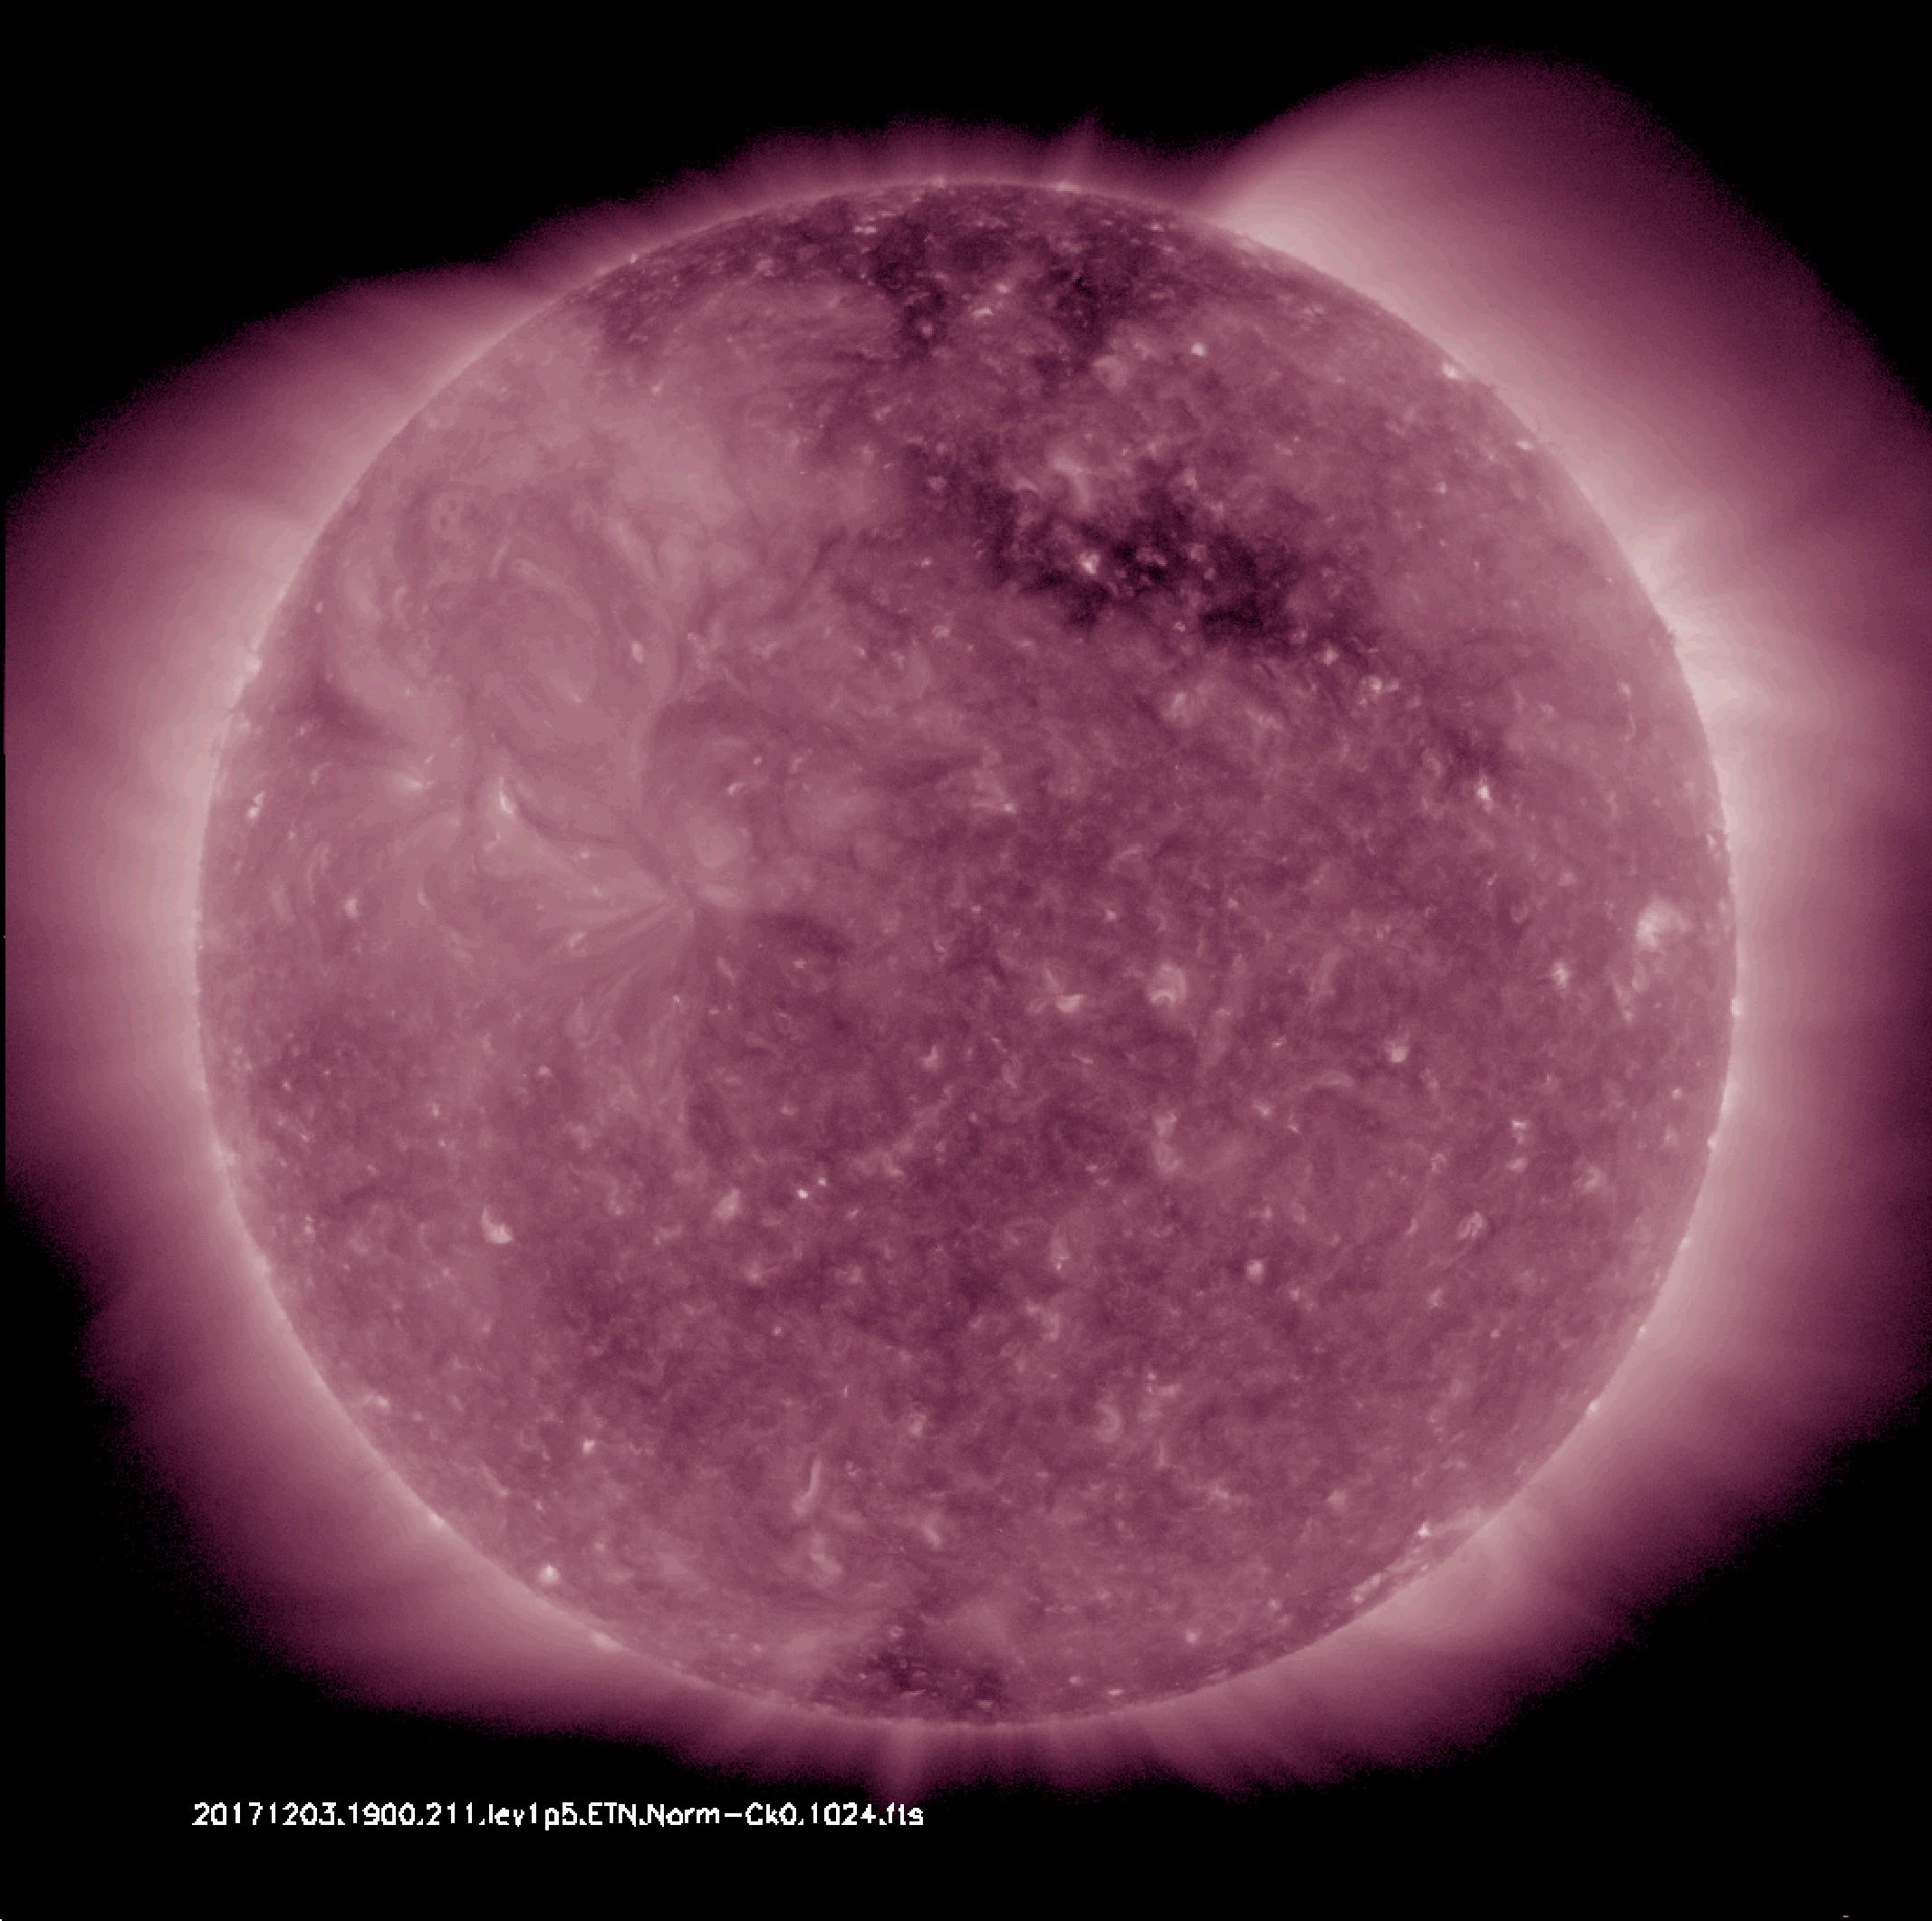
\includegraphics[width=0.95\columnwidth]{img_211.pdf}
  \hskip 0.5cm
  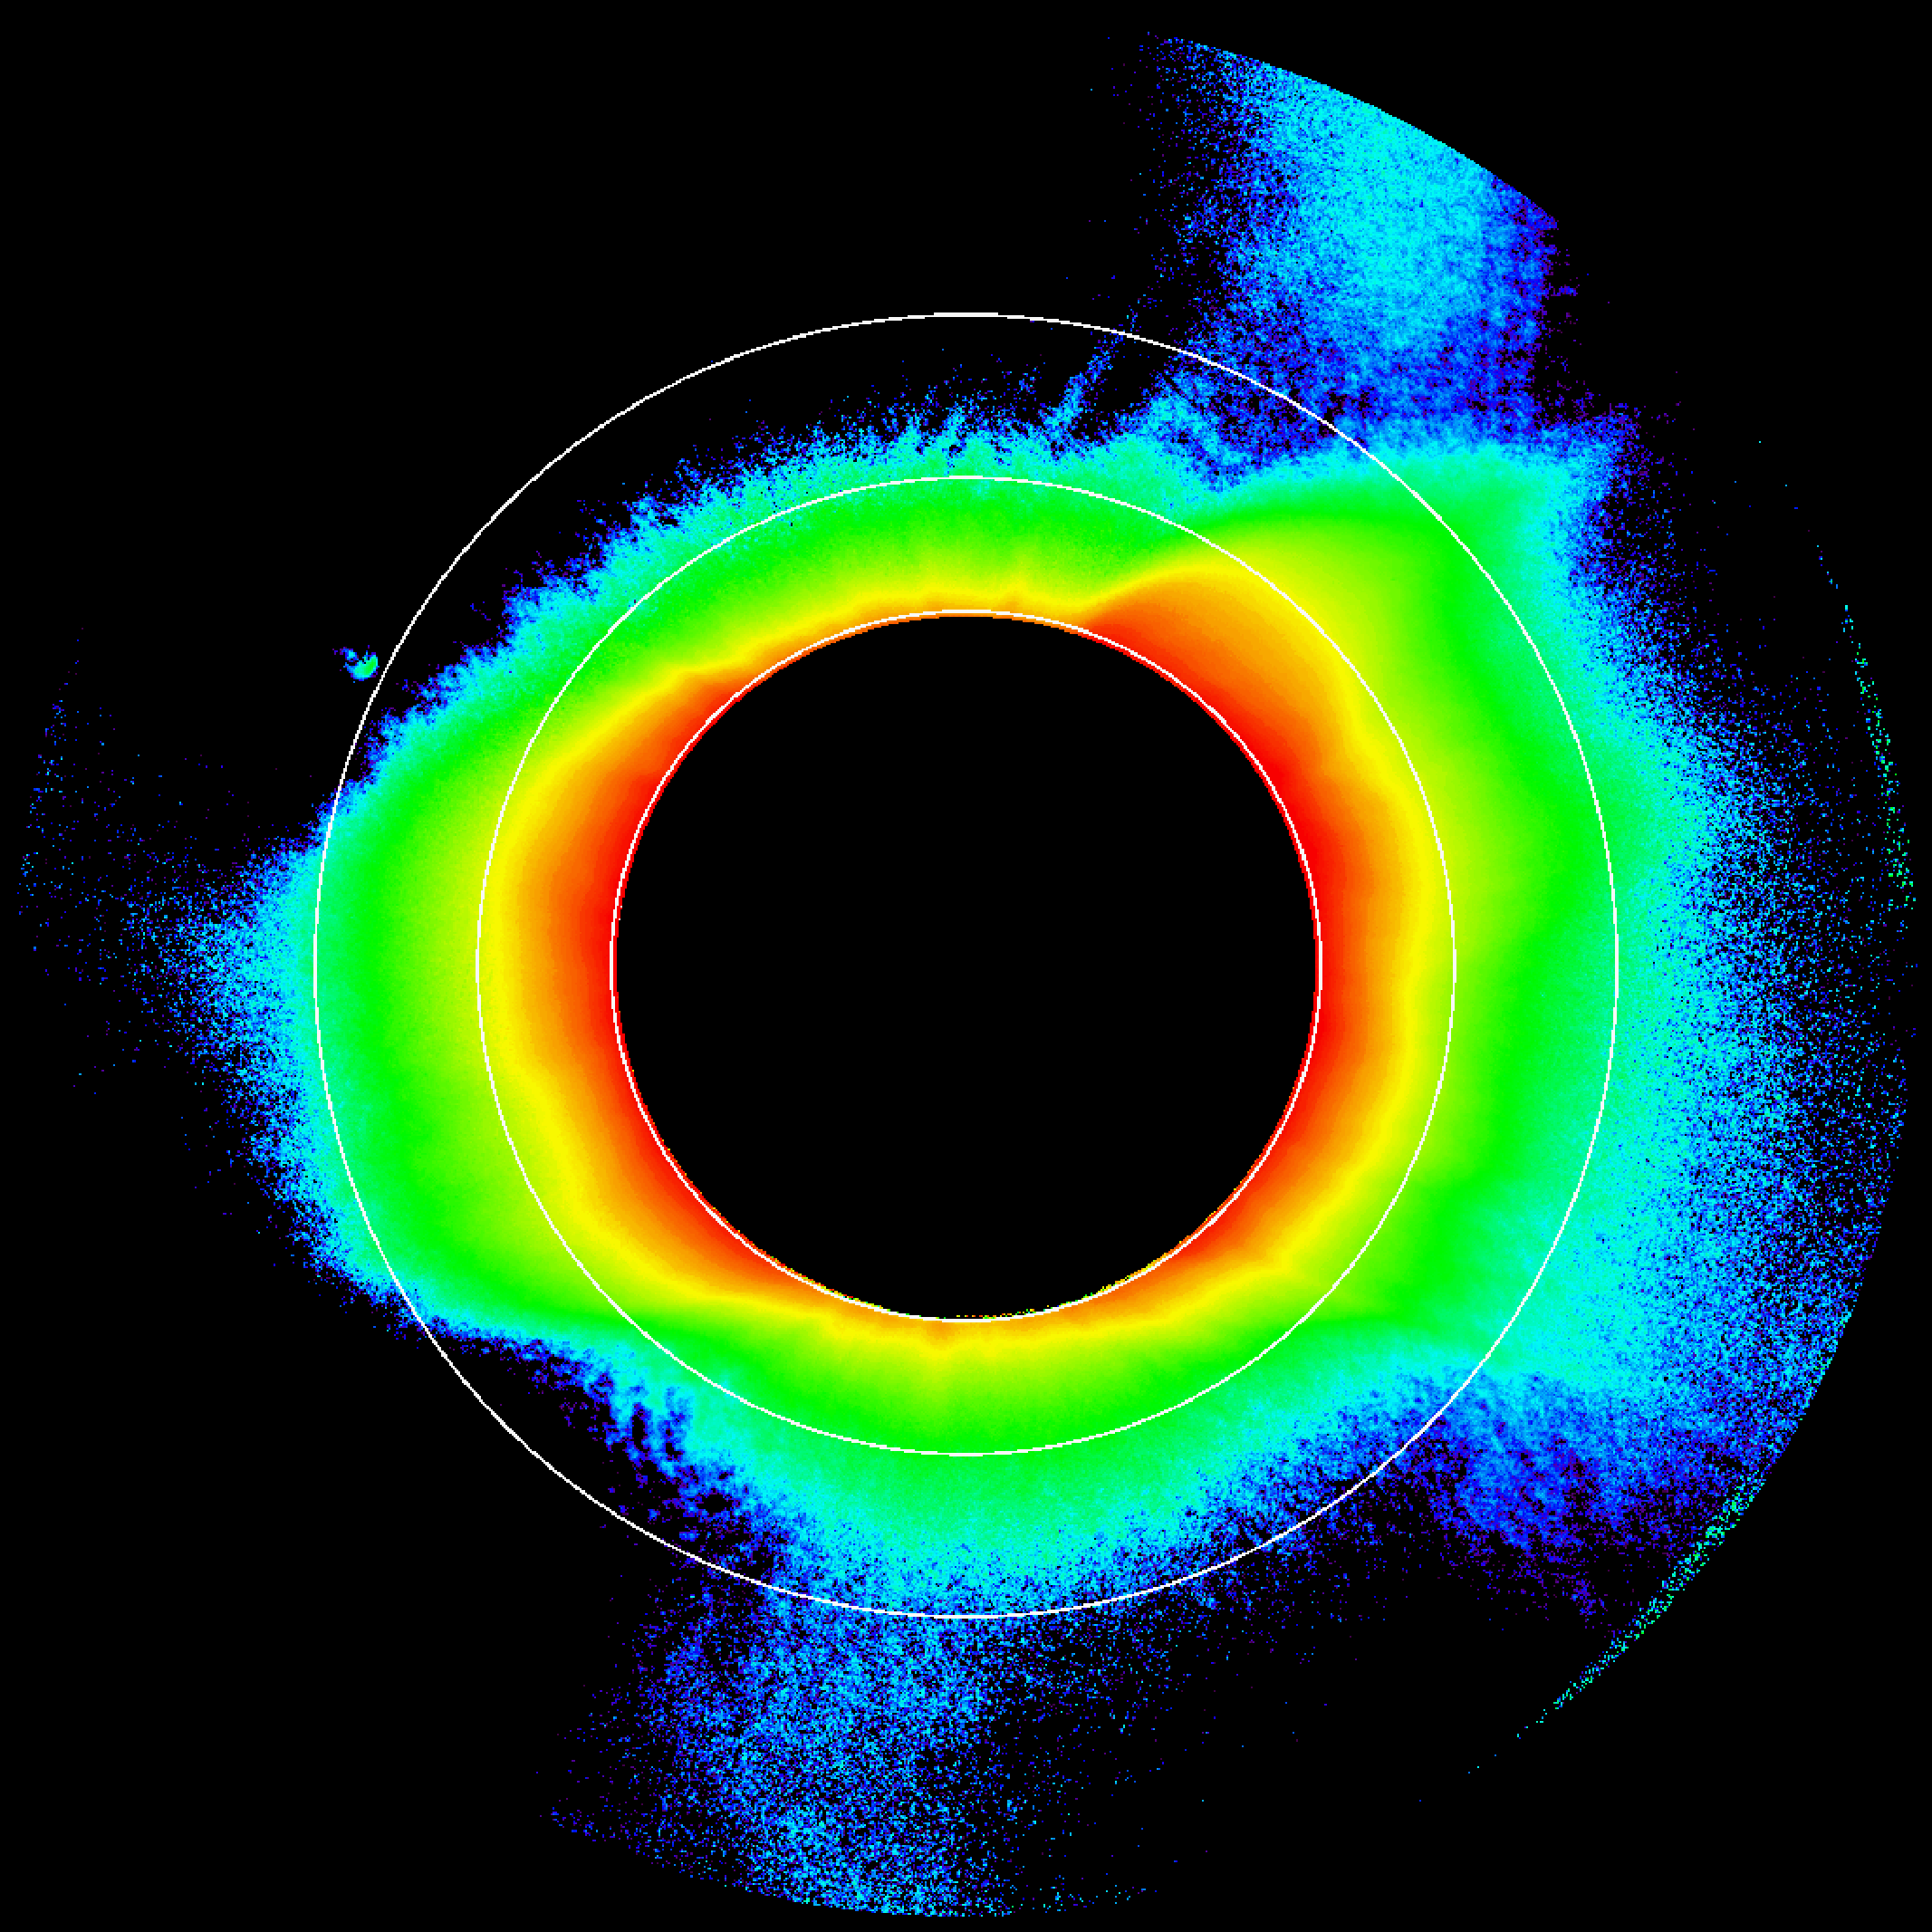
\includegraphics[width=0.95\columnwidth]{20171203_180316_kcor_l1_10min_avg_image.pdf}
  \caption{Example of images used for tomographic reconstruction of the coronal electron density of CR-2198 (see text), both corresponding to 2017 December 03 UT 18:00-19:00. Left panel: SDO/AIA coronal EUV image in the $211~\rm{\AA}$ band. Right panel: HAO/KCOR coronal pB image, with white rings indicating heliocentric heights $1.09, 1.50, \rm{and}\, 2.0~\rm{R}_\odot$.}
  \label{fig_images}
\end{figure*}


\section{Results}

\begin{figure*}[h]
  \centering
  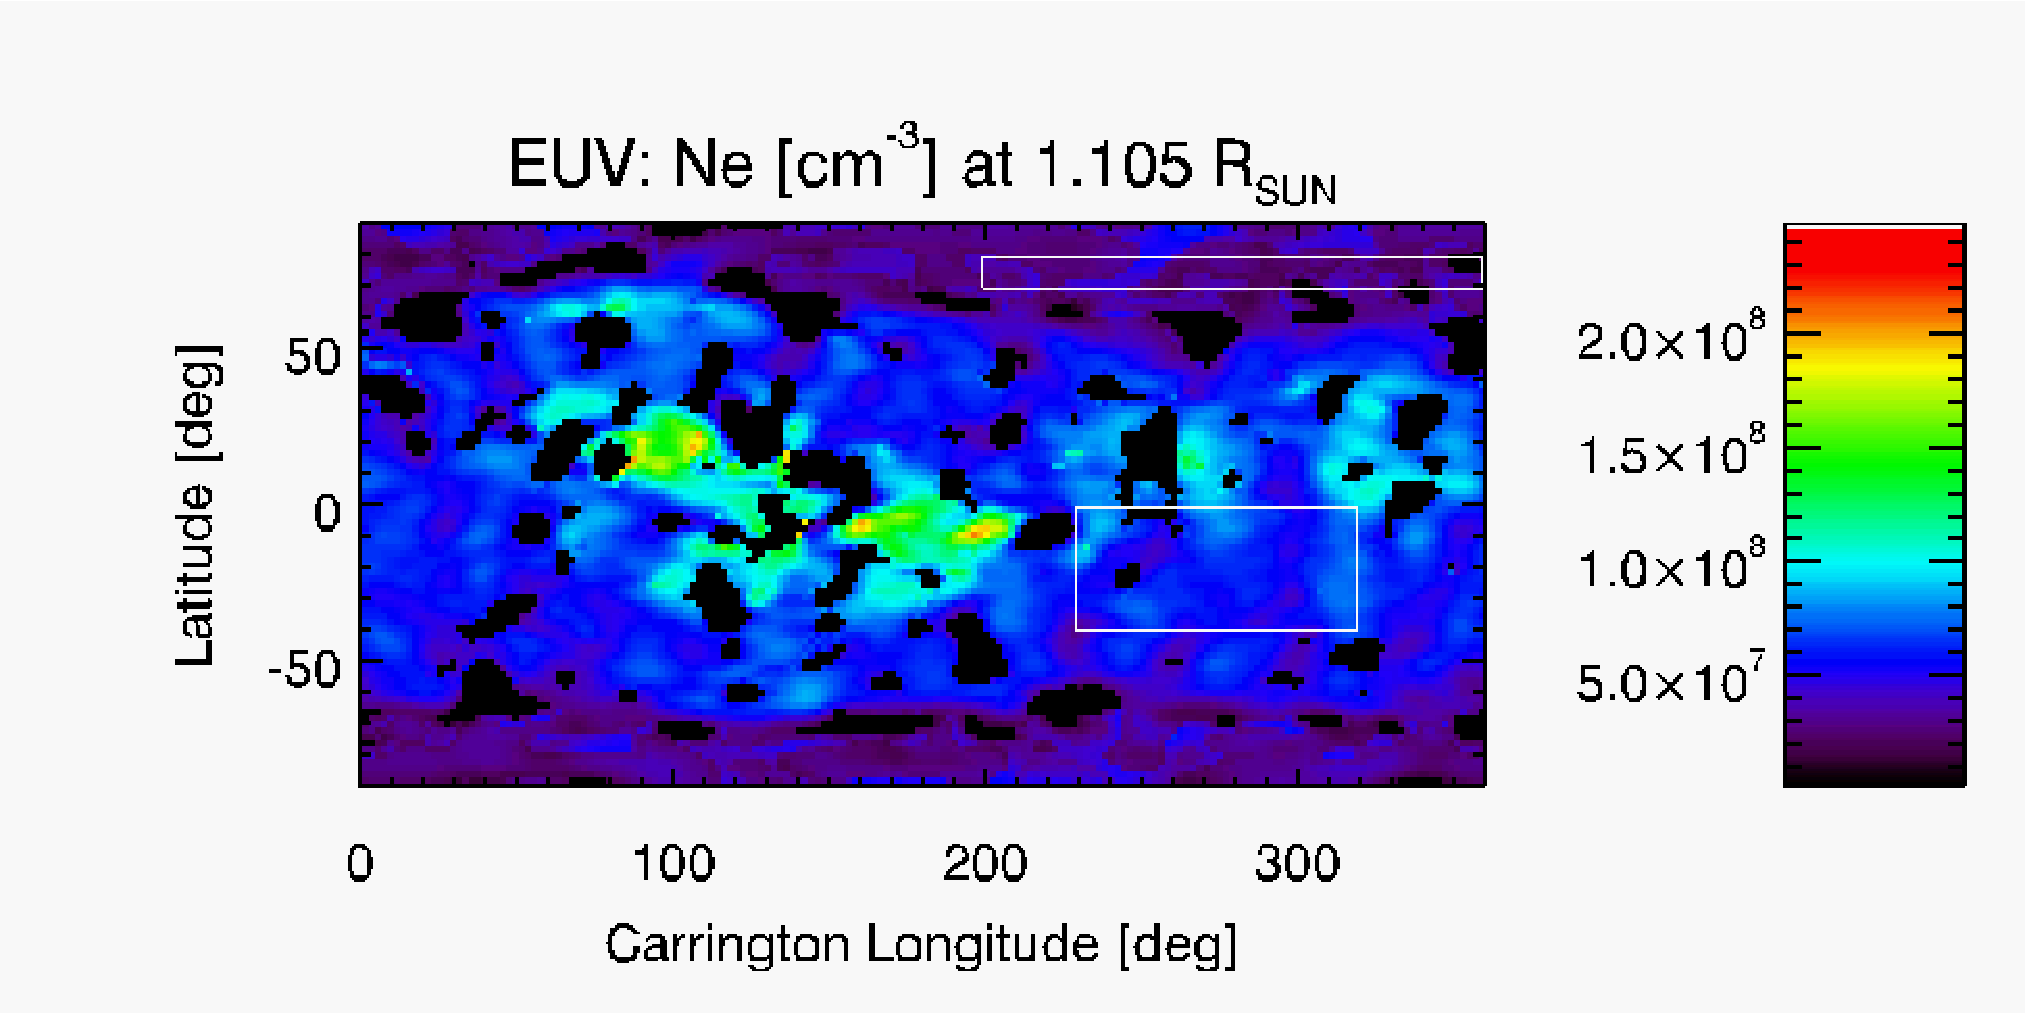
\includegraphics[width=\columnwidth]{map_ne_aia.pdf}
  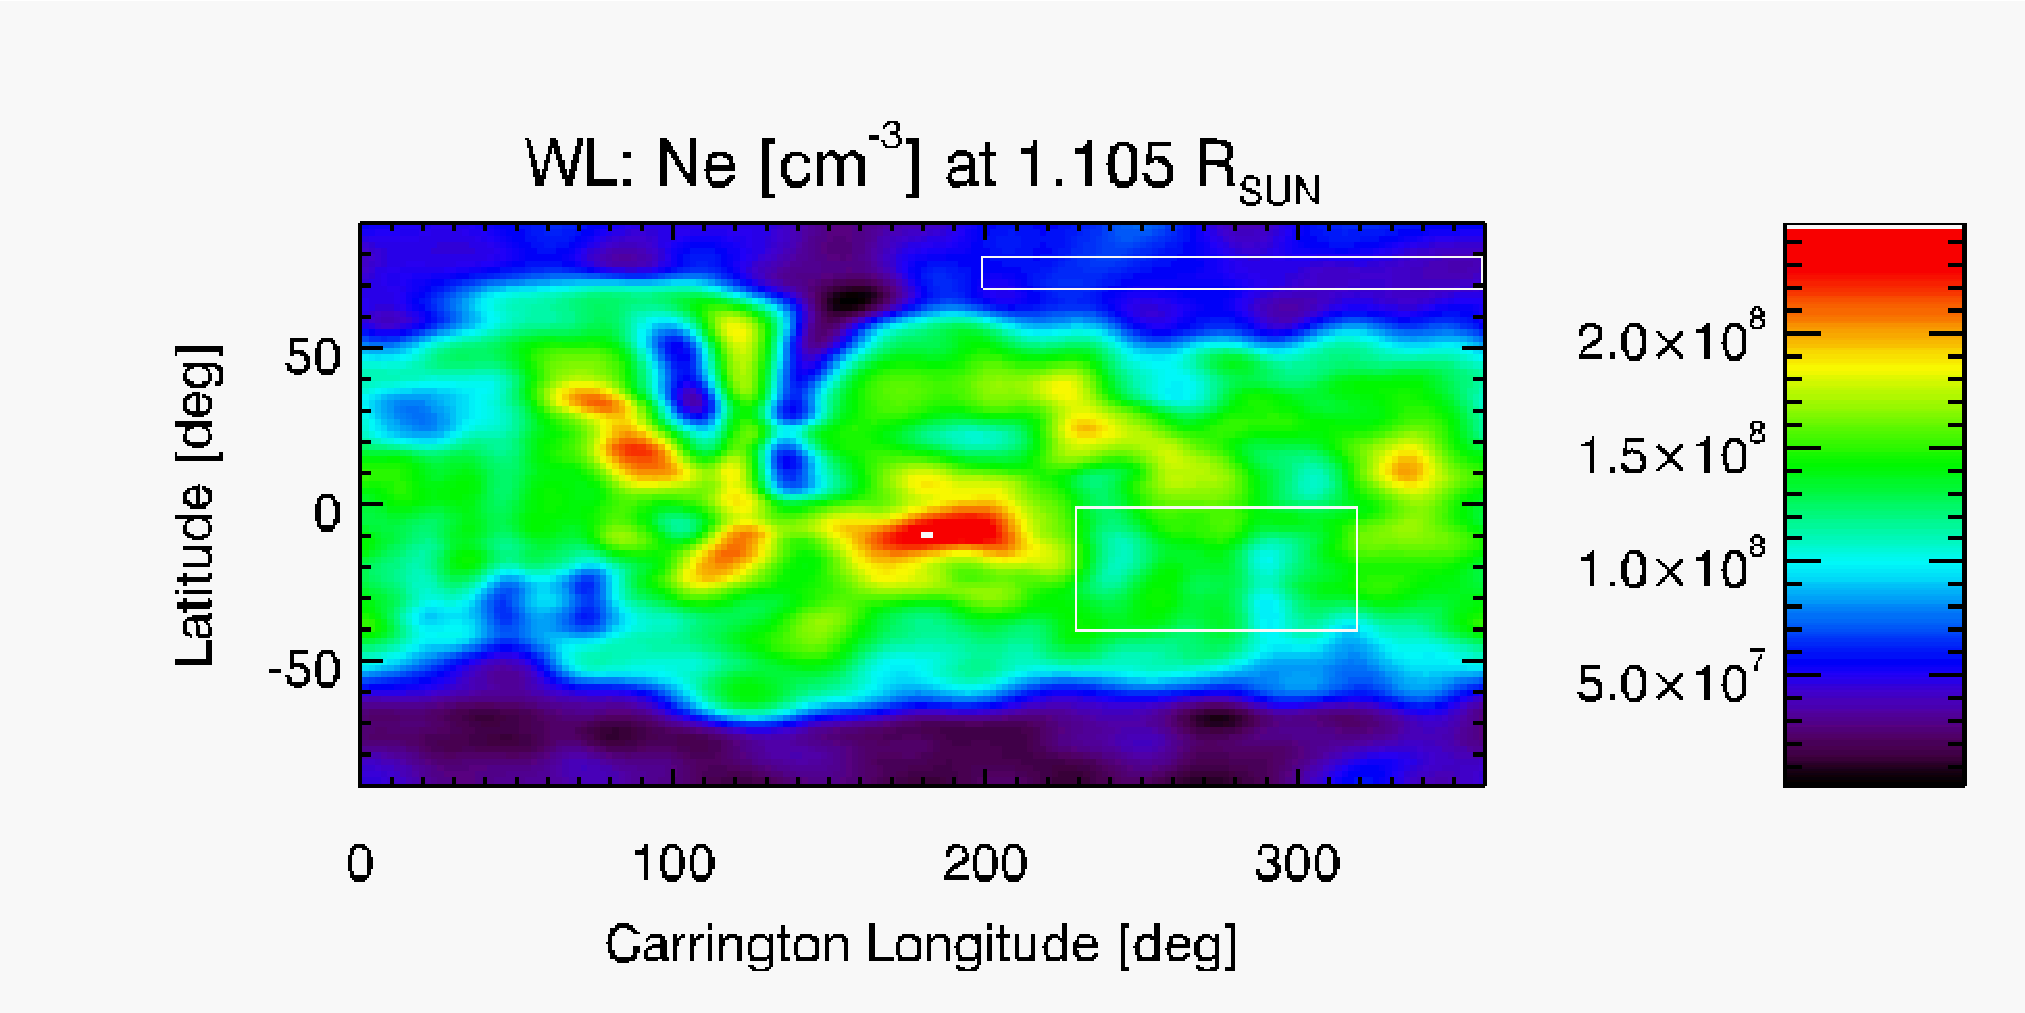
\includegraphics[width=\columnwidth]{map_ne_kcor.pdf}
  \caption{Example of results of the tomographic reconstruction of the electron density of the solar corona for CR-2198. Carrington maps of the reconstructed electron density are shown at heliocentric height $r=1.105~\rm{R}_\odot$. Left panel: reconstruction based on EUV data. Right panel: reconstruction based on WL data. The white boxes indicate two ranges of longitudes and latitudes selected for quantitative comparison. The region in the Southern hemisphere is a high-density quiet Sun region within the equatorial streamer belt during this rotation. The region in the Northern hemisphere is a lower density region at subpolar latitudes in the northern CH.}
  \label{fig_maps}
\end{figure*}

\begin{figure*}[h]
  \centering
  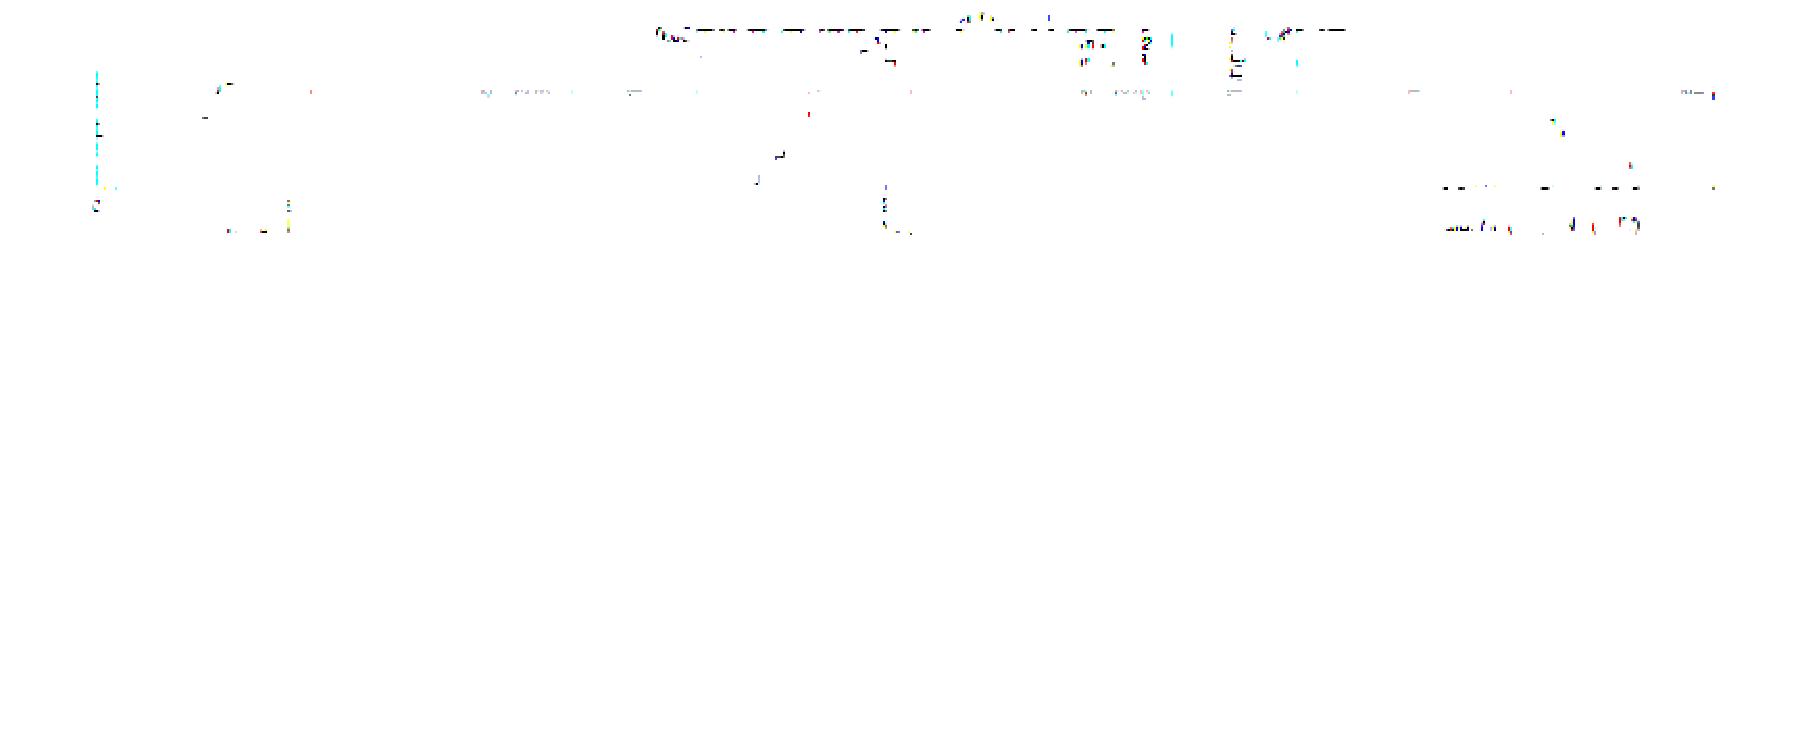
\includegraphics[width=\columnwidth]{comparison_quiet_region.pdf}
  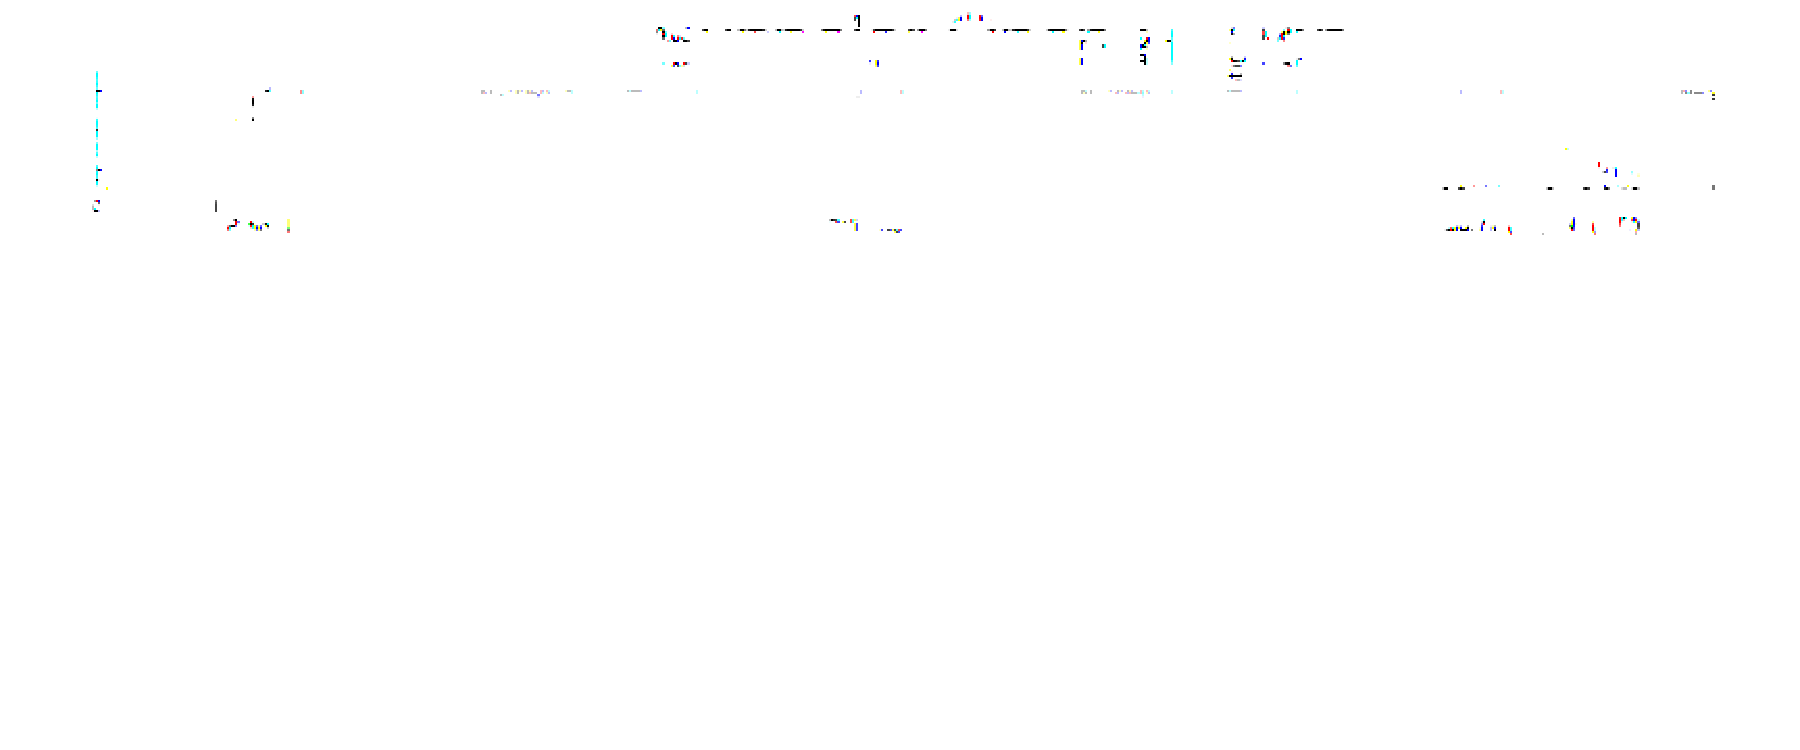
\includegraphics[width=\columnwidth]{comparison_open.pdf}\\
  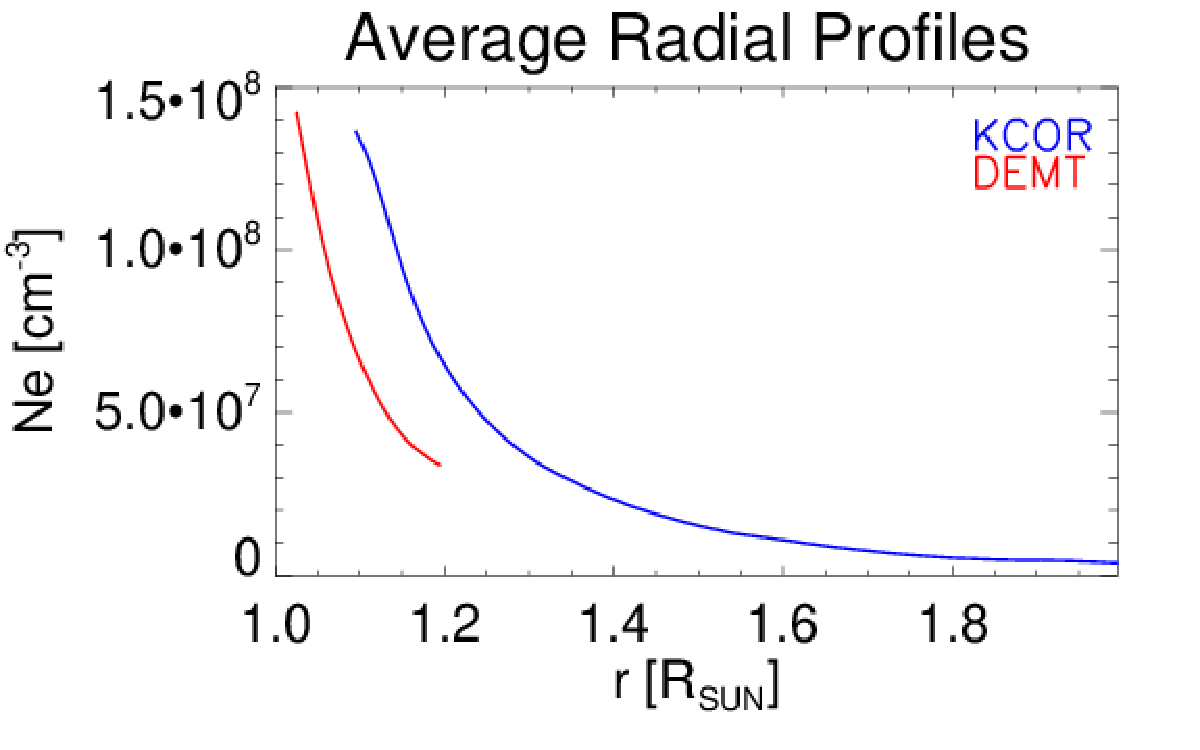
\includegraphics[width=\columnwidth]{Average_Radial_Profiles_KCOR-Tom_vs_DEMT_CR2198_Hh_l45_kcor_subreg-Quiet-region1.pdf}
  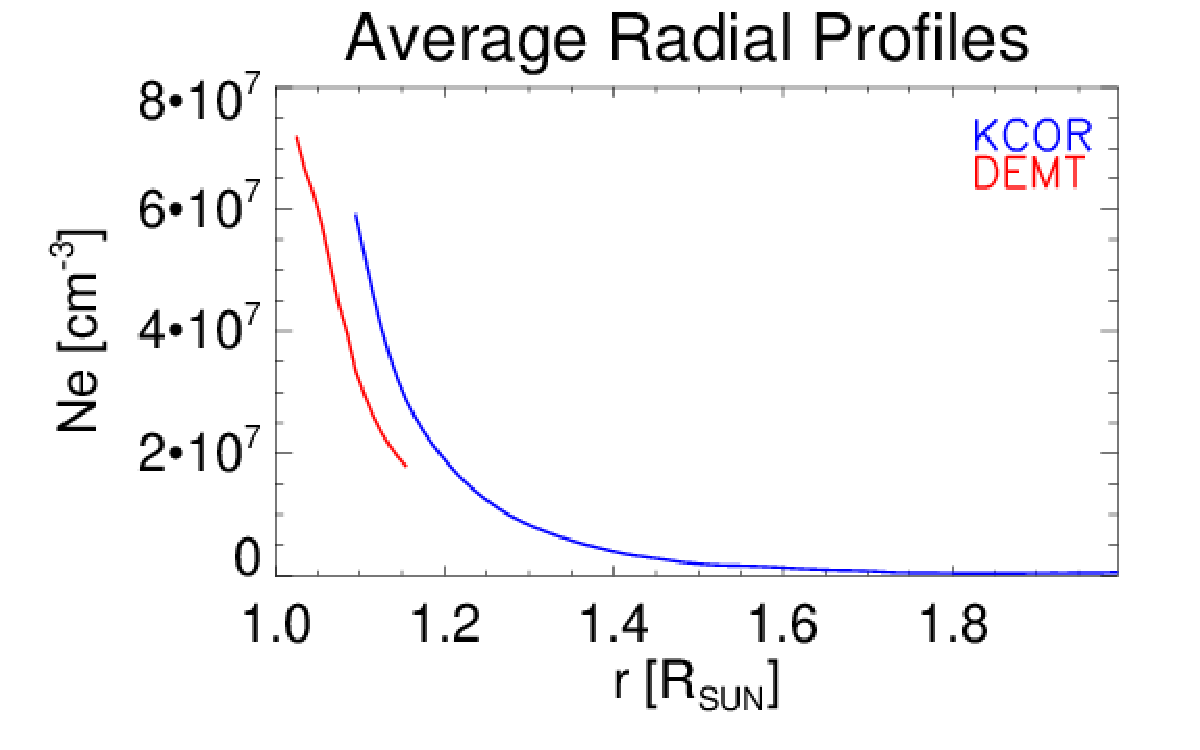
\includegraphics[width=\columnwidth]{Average_Radial_Profiles_KCOR-Tom_vs_DEMT_CR2198_Hh_l45_kcor_subreg-Open-region_N.pdf}
  \caption{Quantitative comparison between the results of the two tomographic reconstructions of the coronal electron density of CR-2198. Results are shown here for the two selected regions indicated in Figure \ref{fig_maps}. Left panels show the results in the quiet sun region of the southern hemisphere within the streamer belt, and right panels show the results in the subpolar open region within the northern CH. For each region, the top panel shows the frecuency histogram of the ratio of the electron density value obtained in each computational voxel from WL and EUV tomographies. For each region, the bottom panels show the average radial profile of the electron density based on the EUV (red) and WL (blue) tomographies.}
  \label{fig_analysis}
\end{figure*}


\section{Conclusions and future efforts}
\begin{itemize}
 \item  $\Eeuv \propto \AvgNE2 = f\,\AvgNe^2$, where \azul{filling factor} is defined as $f\equiv\AvgNE2 / \AvgNe^2$
\salto
\item  $\Ewl \propto \AvgNe$
\salto
\item  Then: $\AvgNe_{\rm{WL}} / \AvgNe_{\rm{EUV}} \propto \sqrt{f}$
\salto
\item  If differences in the results are solely attributed to filling factor:\\
  $f\sim 2$ in subpolar open region, and $f\sim 4$ in quiet sun closed region.
\salto
\item  Note that: $\SigmaNe^2 \equiv \rm{Var}N_e = \AvgNE2 - \AvgNe^2 = \AvgNe^2 \, (f-1)$
\salto
\item  So that: $\SigmaNe / \AvgNe = \sqrt{f-1}$.
\salto
\item  With this interpretation, where $f$ is larger (quiet sun closed region) the electron density probability distribution has larger variance.
\end{itemize}
%%%%%%%%%%%%%%%%%%%%%%%%%%%%%%%%%%%%%%%%%%%%%%%%%%%%%%%%%%%%%%%%%%%%%%%%%%%%%%
%                                                                            %
%  Por favor no modifique las líneas de la bibliografía, salvo el nombre     %
%  el archivo de Bibtex con la lista de citas (sin la extensión .BIB)        %
%                                                                            %
%  Please do not modify the following lines, except the name of the Bibtex   %
%  file (whithout the .BIB extension)                                        %
%                                                                            %
%%%%%%%%%%%%%%%%%%%%%%%%%%%%%%%%%%%%%%%%%%%%%%%%%%%%%%%%%%%%%%%%%%%%%%%%%%%%%% 

\bibliographystyle{baaa}
\small
\bibliography{baaa61a_dglloveras}
 
\end{document}
